\section{Introduction}
\label{sec-intro}

Query independent ranking of scholarly articles has drawn significant attentions from both academia~\cite{Garfield471,ChenXMR07,Zhou07-CoRank,ShenAAAI16,Liang16AAAI,Jiang12-MRank,Waltman2014,TanLMGSW16} and industry~\cite{sem-scholar,g-scholar,Sinha15:MAG}. Generally speaking, a ranking is {\em a function that assigns each entity a numerical score}. Query independent ranking aims to give a static ranking based on the scholarly article data only, and is independent of how well articles match a specific query. Such a ranking plays a key role in literature recommendation systems, especially in the {\em cold start} scenario.

\marked{
In the academic community, the most popular approaches to scholarly article ranking have witnessed a shift from citation count analysis~\cite{Garfield471,Hirsch15112005} to graph analysis~\cite{ChenXMR07,Zhou07-CoRank,Jiang12-MRank,Waltman2014}. These graph-based methods leverage the global structure and interactions of the bibliographic networks, and, hence, are usually better than those based on citation counts only.
%
Besides, efforts have also been made from the industry community, among which Google Scholar~\cite{g-scholar}, Microsoft Academic~\cite{ms-academic} and Semantic Scholar~\cite{sem-scholar} are among the most prominent. More specifically, Google Scholar aims to rank articles in the way researchers do, weighing the full text, where it was published, who it was written by, as well as how often and how recently it has been cited.
%Microsoft Academic considers how often and to which a publication is cited to determine the ranking.
On the other hand, Semantic Scholar proposes to use the citation velocity feature, which is a weighted average of the publication's citations for the last three years.
}

% https://scholar.google.com/intl/zh-CN/scholar/about.html
% http://academic.research.microsoft.com/About/Help.htm
% https://www.semanticscholar.org/faq#citation-velocity




Scholarly articles are involved with multiple entities such as authors, venues, dates and references. Hence, scholarly article ranking is essentially a problem of assessing the importance of nodes in a heterogeneous network.
However, effective and efficient ranking of nodes in such a large complex network is a challenging task since the involved entities
are heterogeneous, evolving and dynamic~\cite{AggarwalS14-survey,fcs-biggraph}.



First, even if we are only to rank one type of entities (\ie scholarly articles), the other types of entities (\eg venues and authors) are closely involved, and, moreover, different types of entities may have different impacts on the ranking of scholarly articles.
%
\marked{Second, the importance of an article varies with time in a complex way~\cite{WangSB13,Chakraborty15}.
%Newly published articles are very likely to have increasing impacts in the next few years, and those published many years ago tend to have decreasing impacts, as researchers potentially have more interests in recently reported results. Indeed, as shown by the statistics of three scholarly datasets (\aan, \aminer and \magdata) in Fig.~\ref{fig-citation}, the citation numbers of articles in general reach the peak in the first 1 or 2 years after their publication, and then decrease accordingly. % Note that we do not plot the proportion of citations at $x=0$ on \aminer, which is an impractical value of 23.6\%. The above citation pattern is described as a complex log-normal probability in~\cite{WangSB13}.
Newly published articles are very likely to have increasing impacts in the next few years, and those published many years ago tend to have decreasing impacts, which conform to the universal pattern of citation profiles such that the number of citation generally grows in the first two to three years, remains at a steady peak of one to two years, and then decline over the rest of time~\cite{Chakraborty15}. Moreover, Chakraborty et al. discuss in~\cite{Chakraborty15} that individual articles indeed follow a remarkable diverse set of patterns (instead of the general one), and categorize all articles into six patterns featured by the time when the numbers of citations reaches the peaks.
}
Finally, academic data is dynamic and continuously growing. Indeed, the number of articles in \magdata has exceeded 126 million, and keeps increasing at around 5.7 million per year~\cite{Sinha15:MAG}. \marked{Such dynamism may possibly cause certain long-term biases into data, \eg the number of citations produced by scholarly articles published in each year increases significantly over time, which should be properly considered. }


Query independent ranking of scholarly articles is challenging~\cite{wsdmcup}, although there exists quite a bit of work on scholarly article ranking, \eg~\cite{Garfield471,ChenXMR07,Zhou07-CoRank,ShenAAAI16,Liang16AAAI,Jiang12-MRank,Waltman2014}.
\marked{Most previous work exploits the time-dependent information of scholarly data in the form of exponential decay~\cite{Li08TSRanking,Wang13AAAI,sayyadi09,WalkerXKM07}, which fails to fit to the diverse citation patterns of individual articles~\cite{Chakraborty15}.}
Further, to our knowledge, little concern has been paid to dynamic scholarly article ranking except \cite{GhoshKHLL11} with a strong and impractical assumption that there are no citations between papers published in the same years.
\marked{Finally, the bias caused by the dynamism of data has never be exploited in scholarly article ranking}.




\eat{
\begin{figure}
\vspace{1ex}
\includegraphics[scale=0.45]{fig/citation.eps}
\vspace{-2ex}
\caption{\small Citation statistics of scholarly articles}
\label{fig-citation}
\vspace{-3ex}
\end{figure}
}

\stitle{Contributions \& Roadmap}.
To this end, we propose an effective and efficient approach for query independent scholarly article ranking in a dynamic environment.

\sstab(1) We first  propose a \underline{S}cholarly \underline{A}rticle \underline{Rank}ing model, referred to as \ensemblerank, by assembling the importance of three classes of entities (articles, venues and authors) for scholarly article ranking (Section \ref{sec-model}).
%
The importance is a combination of {\em prestige} and {\em popularity} to capture the evolving nature of entities.
%
To compute the prestige of articles and venues, we propose a novel {\em Time-Weighted PageRank} with a time decaying factor (based on citation statistics), and the prestige of authors is the average prestige of all their published articles.
%
The popularity of an article is the sum of all its citations' freshness (how close to the current year), while the one of venues and authors is the average popularity of their associated articles.
%
%Observe that (a), intuitively, prestige favors articles with many citations soon after their publication, and popularity favors those with recent citations, and (b) both prestige and popularity capture the evolving nature of entities.
%
\marked{To the best our knowledge, the Time-Weighted PageRank in this work is among the first to incorporate both the diverse citation patterns of individual articles and the bias caused by the dynamism of data to better model the evolving prestige.}


\sstab(2)  We then develop  a batch algorithm for scholarly article ranking (Section \ref{sec-alg}), in which we propose a block-wise method for Time-Weighted PageRank in terms of an analysis of the citation characteristics of scholarly articles.
%
We further develop an incremental algorithm for dynamic scholarly article ranking (Section~\ref{sec-incAlg}), which partitions graphs into  {\em affected and unaffected areas}, and employs different updating strategies for nodes in affected and unaffected areas.


\sstab(3) Using three real-life scholarly datasets (\aan, \aminer and \magdata), we finally conduct an extensive experimental study (Section~\ref{sec-exp}).
(a) We find that our \ensemblerank model improves the pairwise accuracy \cite{Richardson06:BPR} over (\pagerank \cite{Brin98:PageRank}, \futurerank \cite{sayyadi09}, \hhgrank \cite{Liang16AAAI}) by
(11.2\%, 1.8\%, 3.0\%) on \aan,
(6.8\%, 1.8\%, 1.2\%) on \aminer and
(6.5\%, 2.5\%, 1.2\%) on \magdata, on average, respectively.
%
(b) Our batch algorithm \batensemble and incremental algorithm \incensemble are also efficient. Indeed, \incensemble is on average (2.0, 4.1, 229) times faster than (\batensemble, \futurerank, \hhgrank)  on the large dataset \magdata.



\eat{
\stitle{Organization}. The rest of our paper is organized as follows. The latter part of Section~\ref{sec-intro} summarizes related work. Section~\ref{sec-model} introduces the ranking model. Section~\ref{sec-alg} .... Section~\ref{sec-incAlg} .... Experimental results are reported in Section~\ref{sec-exp}, followed by conclusions in Section~\ref{sec-conc}.
}



